% last updated in April 2002 by Antje Endemann
% Based on CVPR 07 and LNCS, with modifications by DAF, AZ and elle, 2008 and AA, 2010, and CC, 2011; TT, 2014; AAS, 2016

\documentclass{llncs}
\usepackage{graphicx}
\usepackage{amsmath,amssymb} % define this before the line numbering.
\usepackage{ruler}
\usepackage[dvipsnames]{xcolor}
\usepackage{subcaption}
\captionsetup{compatibility=false}
\usepackage{xcolor}
\usepackage[width=122mm,left=12mm,paperwidth=146mm,height=193mm,top=12mm,paperheight=217mm]{geometry}
\usepackage{multirow}
\usepackage{algorithm}
\usepackage[]{algpseudocode}
\newcommand{\jason}[1]{\textcolor{orange}{\textbf{JASON: #1}}}
\newcommand{\madan}[1]{\textcolor{red}{#1}}

\begin{document}
% \renewcommand\thelinenumber{\color[rgb]{0.2,0.5,0.8}\normalfont\sffamily\scriptsize\arabic{linenumber}\color[rgb]{0,0,0}}
% \renewcommand\makeLineNumber {\hss\thelinenumber\ \hspace{6mm} \rlap{\hskip\textwidth\ \hspace{6.5mm}\thelinenumber}}
% \linenumbers
\pagestyle{headings}
\mainmatter
\def\ECCV18SubNumber{1816}  % Insert your submission number here

\title{TARP: Tensorflow-based Activity Recognition Platform} % Replace with your title

\titlerunning{TARP: Tensorflow-based Activity Recognition Platform}

\authorrunning{Eric Hofesmann, Madan Ravi Ganesh \and Jason J. Corso}

\author{Eric Hofesmann, Madan Ravi Ganesh \and Jason J. Corso}
\institute{University of Michigan}
\newcommand{\acro}{TARP}
\newcommand{\model}{\textbf{Model submodule}}
\newcommand{\checkpoint}{\textbf{Checkpoint submodule}}
\newcommand{\metrics}{\textbf{Metrics submodule}}
\newcommand{\data}{\textbf{Data Input Block}}
\newcommand{\exec}{\textbf{Execution Block}}

\maketitle

\begin{abstract}
Action recognition is a widely known and popular task that is essential to build up knowledge for video understanding. 
Within the wide research community that take up action recognition challenges, there does not exist a simple and easy-to-use platform that contains a large number of state-of-the-art (SOTA) models and is capable of quickly generating results across multiple datasets.
Given that individual research code is not written with an end user in mind and in certain cases code is not released, even for published articles, the importance of a common unified platform capable of delivering results while removing the burden of developing an entire system is further underlined.
To try and overcome these issues, we develop a tensorflow-based unified platform to abstract away unnecessary overheads in terms of an end-to-end pipeline setup in order to allow the end user to quickly and easily prototype action recognition models.
With the use of a consistent coding style across different models and seamless data flow between various submodules, the platform lends itself to the quick generation of results on a wide range of SOTA methods across a variety of datasets.
All of these features are made possible through the use of a fully pre-defined training and testing pipeline built on top of a small but powerful set of modular functions that handle asynchronous data loading, model initializations, metric calculations, saving and loading of checkpoints, and logging of results. 
The platform is geared towards easily creating models, with the minimum requirement being the definition of a network architecture and preprocessing steps from a large custom selection of layers and preprocessing functions.
\acro~currently houses four SOTA activity recognition models which include, I3D, C3D, ResNet50+LSTM and TSN. 
The recognition performed achieved by these models are, $XX\%$ for ResNet50+LSTM and $YY\%$ for C3D on XXXXX while I3D and TSN achieve $ZZ\%$ and $QQ\%$ on YYYYY respectively.

\keywords{tensorflow, activity recognition, framework, state-of-the-art models, C3D, I3D, Temporal Segment Networks, ConvNet+LSTM}
\end{abstract}

\section{Introduction}
\label{sec:intro}

\section{Overview of \acro}
\label{sec:overview}

\begin{figure}[b!]
\centering
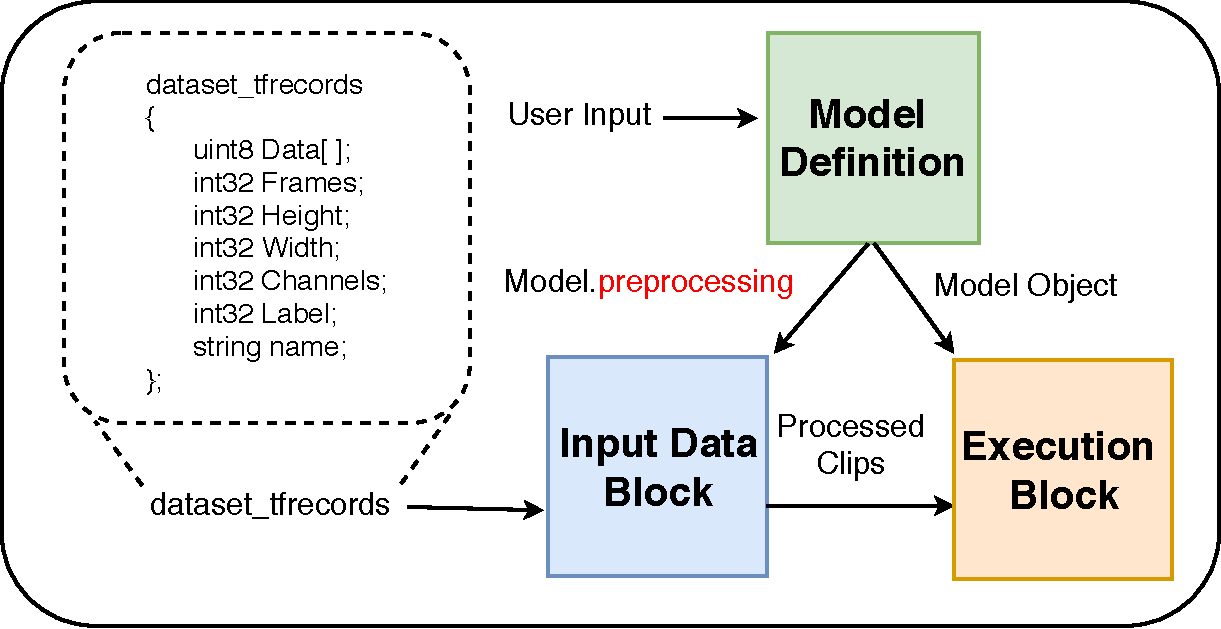
\includegraphics[width=0.8\textwidth]{images/overview.pdf}
\caption{Illustration of the two main components of \acro}
\label{fig:overview}
\end{figure}

\acro~is comprised of two main components, 1) the data input block, and 2) the execution block, as shown in Fig.~\ref{fig:overview}. 
The pipeline contained within the data input block can be divided into three simple stages,
\begin{enumerate}
\item Read video data from disk
\item Extract the desired number of clips from a given video
\item Preprocess the frames of clips using a selected model's preprocessing strategy.
\end{enumerate}
On the other hand, the execution block houses all of the code required to setup, train, test as well as log the outputs of a chosen model.
This includes defining the layers that comprise the model, training the model up to a predetermined number of epochs, saving parameter values of a model are regular intervals and finally testing the performance of the trained model over a variety of recognition metrics.
The following sections provide an in depth discussion of the setup and structure of various components that make up the data input and execution blocks.

\section{Input Pipeline}
\label{sec:ippipeline}
Included in the input pipeline are all of the steps required to pass a video into a model in the proper format.
The three stages of the input pipeline are detailed below.

\subsection{Read video data}
\label{sec:readdata}
When a training or testing instance is run on a model, the first step is to setup the tensorflow graph.
The first node in this graph is the tensorflow tfrecords file reader. 
Video data, stored as tfrecords, are read into the system in a FIFO queue.


\subsection{Extract clips}
\label{sec:extractclips}
Certain models, for example C3D~\ref{}, require their inputs to be in the form of multiple clips extracted from a single video.
To allow for the loading of multiple clips for each loaded video, another FIFO queue is added to the pipeline to store individual clips.
Fig.~\ref{fig:extract_clips} details the data flow from the tfrecords video data queue, through the clip extraction algorithm, and into the clips queue.
By default, the clip extraction algorithm is set to process and entire video at a time and only extract clips if the required arguments have been specified.

\begin{figure}[b!]
\centering
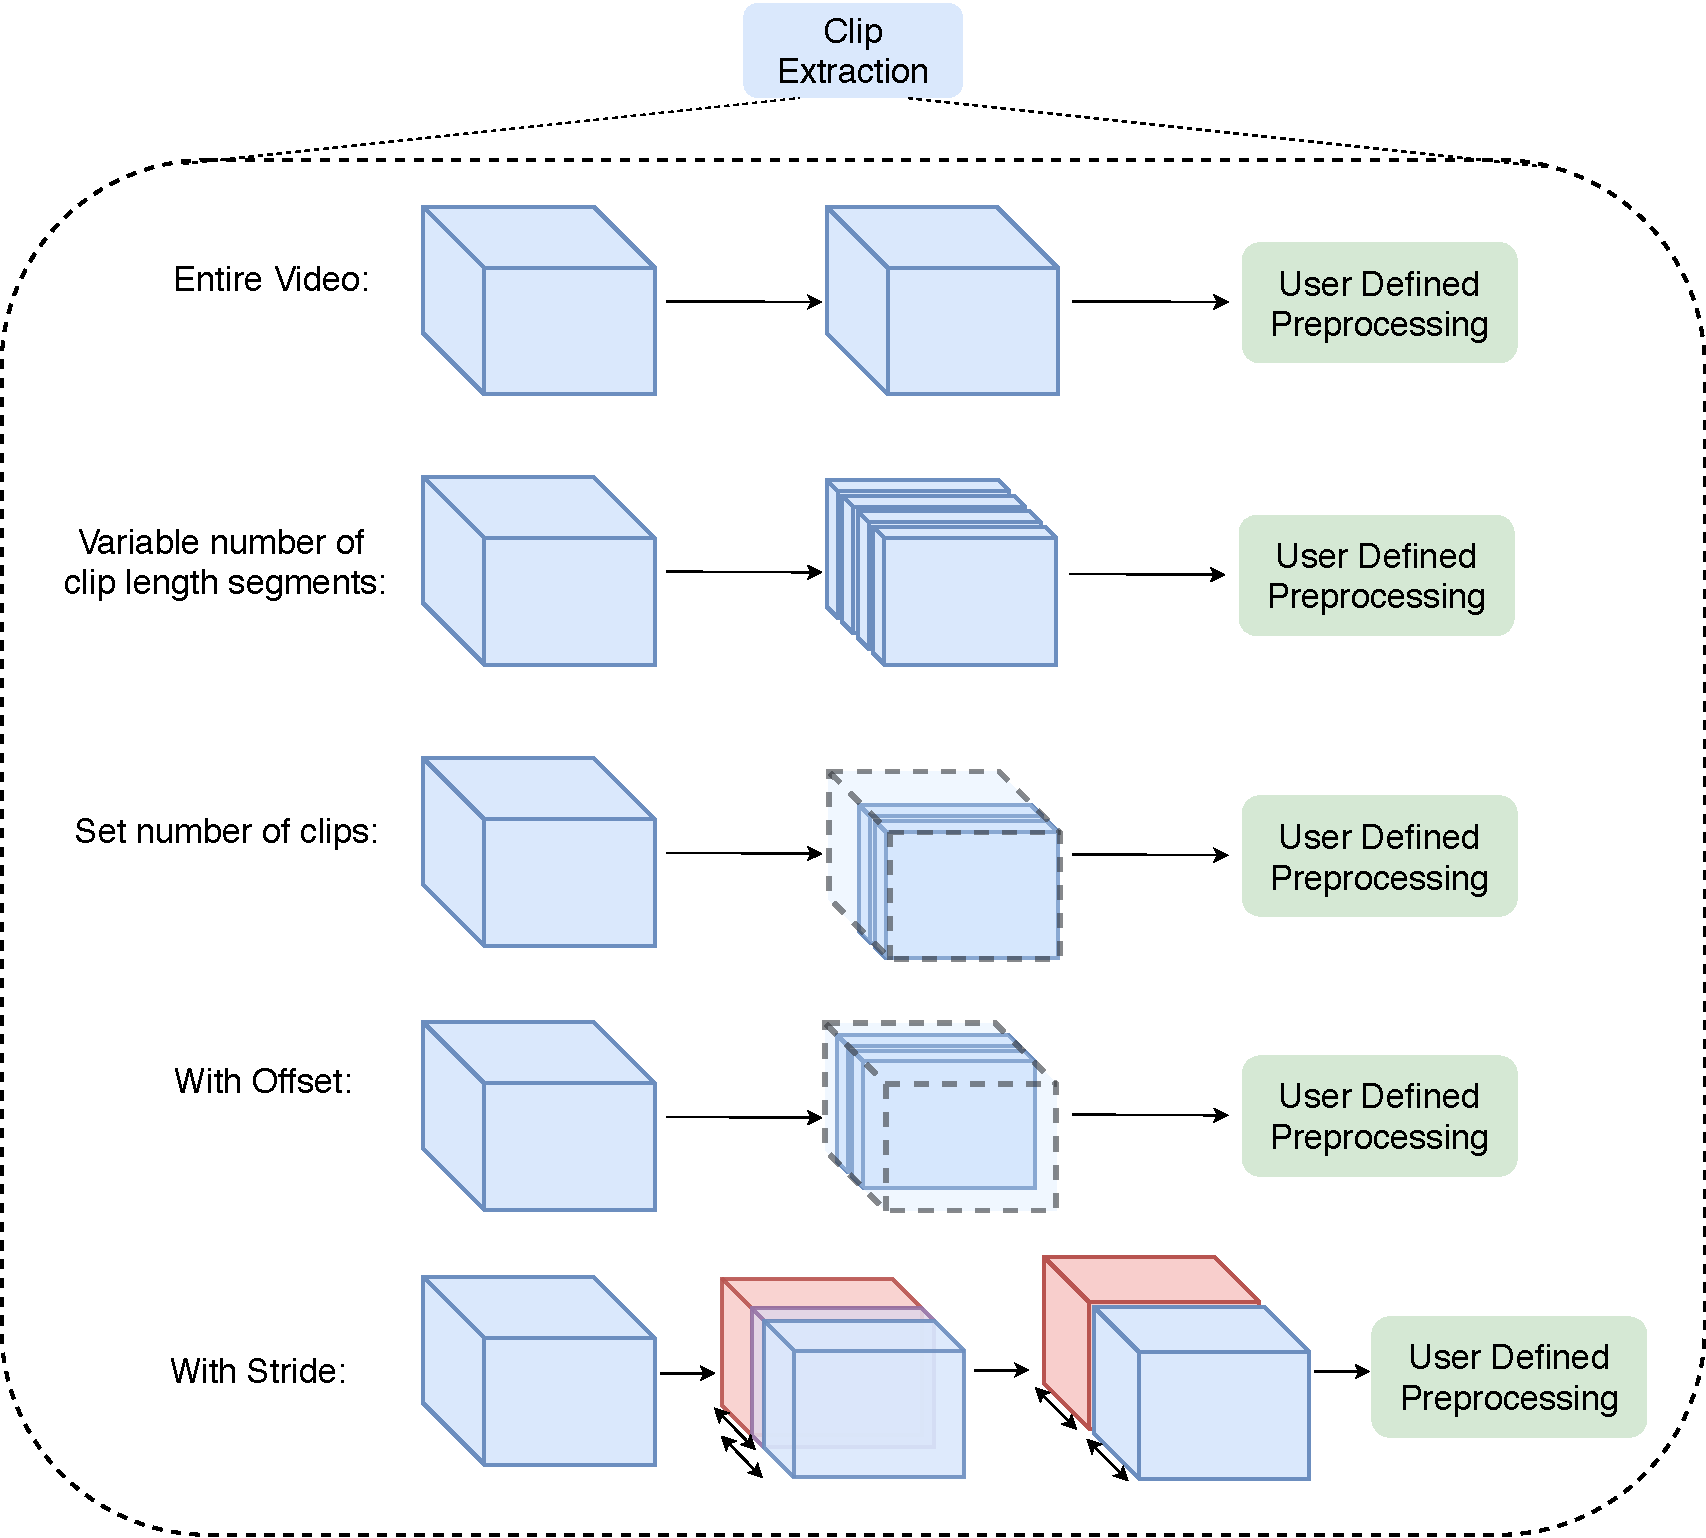
\includegraphics[width=0.8\columnwidth]{images/extract_clips.pdf}
\caption{The input pipeline allows for videos to be broken into clips according to defined specifications.
Whenever a video has been completely processed and used for training or testing, a new video is loaded from the queue.
The video is then passed through our clip extraction algorithm which enqueues the clips individually into a secondary queue.
Clips are then dequeued from the clips queue according to the number of GPUs being used and the required clip batch size.}
\label{fig:extract_clips}
\end{figure}


\subsection{Preprocess clips}
\label{sec:preprocessclips}
Activity recognition employ a number of various preprocessing methods on a frame or clip-based level.
These can include frame-wise cropping, flipping, and resizing, or clip-wise temporal offsets, resampling, and looping.
In order to incorporate these methods as desired per model, we create one or multiple preprocessing files for each model.
The desired preprocessing file for a model can be defined within the model and then called from the inputs call 

\acro~includes implementations of all of these options which can easily be added to a model's preprocessing file.



\section{Execution Block}
\label{sec:execblock}
The execution block form the largest component of the entire platform. Its code can be broken down into parts that are used during two alternate phases, training and testing.
Fig.~\ref{fig:exec_block} illustrates this concept and highlights the submodules used within each phase.
An algorithmic overview of each phase, followed by a detailed description of the various submodules used within them are provided in the following sections.

\begin{figure}[t!]
\centering
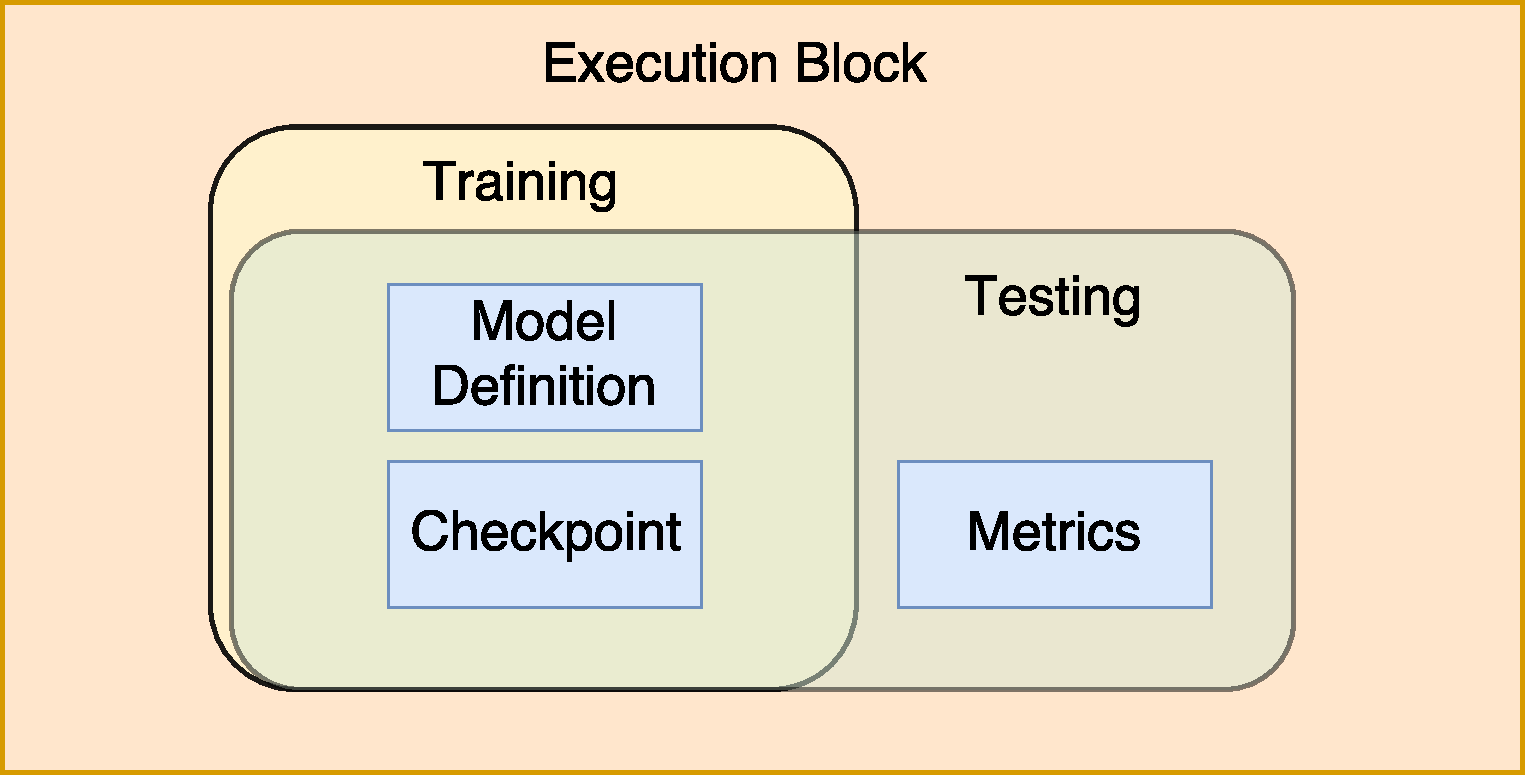
\includegraphics[width=0.8\columnwidth]{images/exec_block.pdf}
\caption{Training and Testing functions are the two major phases within the execution block. Model definitions and checkpoint-based functions are part of both training and testing functions while metrics are calculated after models are tested.}
\label{fig:exec_block}
\end{figure}

\subsection{Training: Algorithmic flow of processes}
\label{sec:training}
Training, within the context of the execution block, follows the process flow outlined in Alg.~\ref{}.
The beginning of every training phase is associated with the selection and set up of a model. 
Basic model parameters such as input/output data dimensions, batch normalization, dropout rate, and etc. are passed into the \model~for this purpose.

Once the model has been set up, the next step is to ensure that the parameter weights for the chosen model are retrieved. 
If the model has been pre-trained using \acro~and the user desires to further fine-tune the model, then the model parameter's weights from the latest checkpoint will be restored.
By default, the standard pre-trained weights are loaded into the model.
Alternatively, a random initialization option, for users to train a model from scratch is also provided. 
As a backup when a specified checkpoint is unavailable, the system defaults to the random intialization option, with an additional warning provided to the user about the setup being used.

After the preparation of the model is complete, data tensors are retrieved from the \data~ and interfaced to the model.
The main data retuned from \data~are the video frames, their corresponding labels and video names.
With the availability of the model and data, the next step is to create a copy of the model on each of the selected number of GPUs within a compute node.
Within each GPU, the inference function of \model~is used to generate a copy of the layer definitions. 
Here, the variable names are re-used to ensure that the same copy of weights are associated throughout all the GPUs.
\acro~only supports the extension of a model within a compute node of a cluster. 
Currently, it cannot be distrbute a model across mutiple nodes or split a model across multiple GPUs within a node.

From each of the model copies, we retrieve a desired layer's output. 
Given that the most common approach to training a network is through the use of logits returned from the final layer, we use the variable logits, associated with the last layer, to obtain a loss value.
Finally, the loss and gradients, computed from the loss, across all the model copies are accumulated into the loss\_array and gradients\_array respectively.
The contribution of each model copy is weighted equally and the final gradient used to update the weights of the model is obtained by taking the average of value stored in the gradients\_array.
The is the final stage in the definition of the tensorflow graph required for training.

\begin{algorithmic}[H]
\Procedure{Training}{}
\State \textbf{Model\_definition}.\textcolor{red}{setup}(model\_params)
\State \textbf{Checkpoint}.\textcolor{red}{load\_param\_weights}(default or specific file)
\State Data, Labels = \textbf{DIB}.\textcolor{red}{load\_data}(expt\_params)
\\
\For{each GPU within given node}
\State \textbf{Model\_definition}.\textcolor{red}{inference}(Data, model\_params)
\State tower\_loss = \textbf{Model\_definition}.\textcolor{red}{loss}(Labels, returned\_logits)
\State tower\_gradients = gradients(tower\_loss)
\State loss\_array.store(tower\_loss)
\State gradients\_array.store(tower\_gradients)
\EndFor
\\
\State grad = average\_gradients(gradients\_array)
\State train\_op = apply\_gradients(grad)
\\
\While{no\_videos\_loaded \textless~(total\_epochs $\times$ videos\_in\_dataset)}
\State \textbf{Checkpoint}.\textcolor{red}{save}() @ regular intervals
\State sess.run(train\_op)
\State update(no\_videos\_loaded)
\EndWhile
\EndProcedure
\end{algorithmic}

After the tensorflow graph for training has been defined, the next step is to execute the graph. 
Usually, models are trained for a typical number of epochs, iterations over the entire dataset.
Within each epoch, based on a set frequency of iterations, we save the model parameter's weights using \checkpoint.save().
The main operation that gets executed within each iteration is the training operation that links the calculation of losses, gradients and their application.
It is important to note that during the setup of the experiment, \acro~ offers adaptive learning rate control which steps down the learning rate when the loss plateaus.
The repeated application of train\_op forms the most crucial and final step in the training process flow.

\subsection{Model Description Submodule}
\label{sec:modeldesc}
\begin{figure}[b!]
\centering
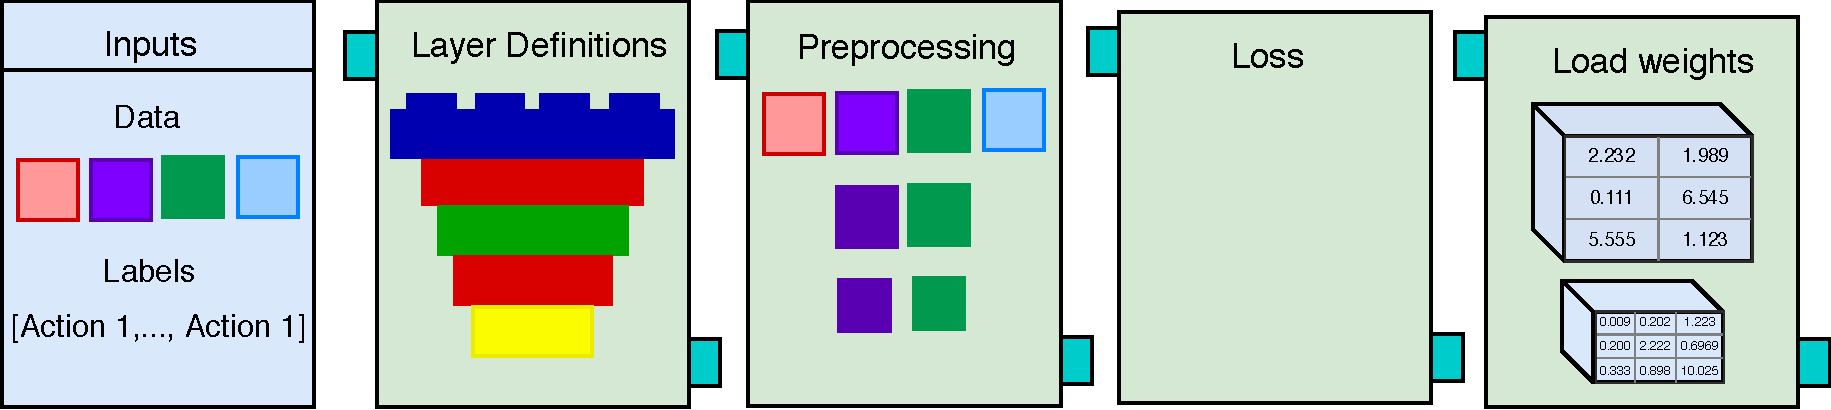
\includegraphics[width=\columnwidth]{images/model_submodule.pdf}
\caption{}
\label{fig:model_submodule}
\end{figure}

The class definition of a model within \acro~can be divided into four main components as shown in Fig.~\ref{}. 
Preprocessing is the first module in the \model that gets used within \data.
In keeping with the modular design paradigm, we use individual functions to define each variant of the preprocessing pipeline.
By keeping each variant within its own file, marked with the suffix ``\textcolor{blue}{\_preprocessing.py}'', we increase their reusability and ensure debugging them is easy.
Within the class definition of a model, multiple preprocessing pipelines can be included using a simple \textit{if-else} construct.
The expected final product from any preprocessing function is the complete preprocessed input data that needs to be passed into a network's input layer.

The definition of a model's input layer and the subsequent layers that make up the model's network architecture should be present within the \textcolor{red}{inference} function.
The layers used must strictly be called from within the set of definitions provided within the \textcolor{blue}{layer\_utils} file.
This ensures that layer definitions are not specific to any network and become available to all models defined within \acro.
Further, it is essential that the inference function returns the outcome of any and all desired layers from within the defined network.
Any accompanying functions to help quickly and/or recursively define a network can be added outisde of the inference function.


As a minor deviation from standard practices, we attach the definition of a loss to the model definition instead of the main training file.
We do this to avoid cluttering and increasing the complexity of the main training file.
Thus, a prime requirement within any model definition is the implementation of a loss function, with the expected return from this function being the final loss value.
To add further flexibility in using multiple losses with a single model, the basic loss function can alternatively be overloaded to call different losses using the internally defined \texttt{\textcolor{ForestGreen}{loss\_type}} keyword.

The final and optional component of any model definition within \acro~is the definition of the \textcolor{red}{load\_default\_weights} function.
This function is defined to ensure that a predetermined set of weights can be loaded into a network's layers.
The explicit rules required to define the layer names and ensure their respective weights can be assigned are provided in Section~\ref{sec:checkpoint}.
The final values returned by this function are the parameter weights loaded from an external file. 

Given that the focus of \acro~is to help the end-user quickly define and integrate a model to the framework, we provide a template file named \textcolor{blue}{models\_template.py} which provides the outline for the user to quickly fill out the inference, preprocessing, loss and load weights functions.
A separate file named \textcolor{blue}{models\_preprocessing\_template.py} provides an outline of the necessary function to defining the preprocessing pipeline.
Once a model has been completely defined, it is automatically imported into the framework through a recursive call strategy.
To quickly track and log a model class variable an inbuilt dictionary named \texttt{\textcolor{ForestGreen}{track\_variables}} is available.
Adding any pre-defined variable name and graph title allows the logging of the desired variable on tensorboard.

Note: 1) Any model defined must be placed within the models folder under a directory with the same name as that of the model,
2) The actual model file must be named with a suffix ``\textcolor{blue}{\_model}''.
2) No explicit model class attributes can be added to a specific model. Instead, they must be added to the \textcolor{blue}{model\_abstract.py} file and made available to any and all model definitions within \acro.

The models that come standard with \acro~include the state-of-the-art activity recognition architectures I3D~\cite{}, C3D~\cite{}, ResNet50~\cite{}, and TSN~\cite{}.

\subsection{Checkpoint Submodule}
\label{sec:checkpoint}
The checkpoint submodule contains utility functions that handle all the essential functions w.r.t. checkpoints. 
Checkpoints themselves are stored in a custom format as shown in Fig.~\ref{}. 
This format readily lends itself to a recursive access strategy while offering easy conversion capabilities from its native numpy format to ``\textcolor{blue}{.ckpt}'',``\textcolor{blue}{.caffemodel}'' and other formats.
Among the variety of operations that can be performed on and using checkpoints, there are two broad categories, Load/Save and Tensor handling.

\paragraph{Load/Save} 
At the beginning and end of every training processes, the ability to save and recover the current/last known state of the model parameters is paramount.
In order to save the current state of a model's parameters, a new checkpoints folder is generated in the results directory.
The folder structure generated to save the checkpoints is, \textless dataset\textgreater/\textless preprocessing\_method\_name\textgreater/\\\textless experiment\_name\textgreater/\textless metric\_name\textgreater/checkpoints. 
Within this folder three distinct files are generated.
\begin{itemize}
\item Checkpoint file: A replica of the checkpoint file obtained from native tensorflow code is generated by the \textcolor{red}{save\_checkpoint} function. 
The current global step is saved within this file, named ``\textcolor{blue}{checkpoint}''.
\item Data file: A separate data file is used to store the current learning rate of the experiment.
The file is named using the convention \textcolor{blue}{checkpoint-\textless global step number\textgreater .dat}. 
\item Numpy weights file: Variables declared and available within the global scope of the experiment are retrieved, name and value, and stored within the numpy weights file. 
It follows a similar naming convention to the Data file, \textcolor{blue}{checkpoint-\textless global step number\textgreater .npy}.
\end{itemize}

When a checkpoint is being loaded, the utility searches for each of the three files defined above to return a distinct variable holding the contents of the files.
If any of the files are missing, the checkpoints fails to get loaded and it is a clear indication of a corrupted checkpoint.

\paragraph{Tensor Handling}
The tensor handler is a recursively defined function which takes names of tensors from the numpy file and loops over assigning the corresponding values associated with those tensor names through the function \texttt{\textcolor{ForestGreen}{tf.assign(tf.graph.get\_tensor\_by\_name(\textless tensor\_name\textgreater), numpy value)}}.
A model is initialized from a pre-existing numpy dictionary through the use of a depth first search and assign policy using the tensor handler. 
An example of this is shown in Fig.~\ref{}.

An important rule for the definition of any tensor name is that the name must explicitly use the terms ``\texttt{\textcolor{ForestGreen}{kernel}}'' and ``\texttt{\textcolor{ForestGreen}{bias}}'' to denote the \texttt{W} (weight) and \texttt{b} (bias) matrices respectively.
No other name is recognized within the framework.

\subsection{Testing: Flowchart of processes}
\label{sec:testing}

\subsection{Metrics Submodule}
\label{sec:metrics}

\section{Benchmarks}
\label{sec:benchmarks}

\clearpage

\bibliographystyle{splncs}
\bibliography{egbib}

\end{document}

\grid
\grid
\grid
\grid
\grid


